\documentclass[aspectratio=169,10pt]{beamer}
\usepackage{issa}  % place issa.sty in the same folder
\definecolor{AccentCol}{HTML}{AD1457}
\renewcommand{\lecnum}{7}
\title{AI \& Machine Learning in Warfare}

% pixel cell: \pc{x}{y}{value 0..9}
\newcommand{\pc}[3]{%
 \pgfmathsetmacro{\shade}{int(100-#3*100/9)}%
 \fill[black!\shade!white] (#1,#2) rectangle ++(1,1);
 \draw[ISSAgrey!60,line width=0.3pt] (#1,#2) rectangle ++(1,1);
 \node[font=\scriptsize,text=\ifnum#3>4 ISSAdark\else white\fi] at (#1+0.5,#2+0.5) {#3};}
% heat cell: \hc{x}{y}{weight 0..1}{label}
\newcommand{\hc}[4]{%
 \pgfmathsetmacro{\pct}{int(round(100*#3))}%
 \fill[AccentCol!\pct!white] (#1,#2) rectangle ++(1,1);
 \draw[white,line width=0.8pt] (#1,#2) rectangle ++(1,1);
 \node[font=\scriptsize,text=\ifdim #3pt>0.5pt white\else ISSAdark\fi] at (#1+0.5,#2+0.5) {#4};}
% plain number cell with border
\newcommand{\nc}[3]{\draw[ISSAnavy,line width=0.4pt,fill=white] (#1,#2) rectangle ++(1,1); \node[font=\scriptsize] at (#1+0.5,#2+0.5) {#3};}
% the 6x6 image (row 0 = top)
\newcommand{\imagegrid}{%
 \foreach \r/\vals in {0/{0,0,0,0,0,0},1/{0,0,0,0,0,0},2/{0,0,9,9,9,9},3/{0,0,9,9,9,9},4/{0,0,9,9,9,9},5/{0,0,9,9,9,9}}{%
  \foreach \v [count=\c from 0] in \vals {\pc{\c}{5-\r}{\v}}}}

\begin{document}
\titleslide{7}{Convolutional Neural Networks}{Filters, feature maps, pooling and the architectures that taught machines to see --- from pixels to target recognition\\Case study: SAR target recognition with a 93,962-parameter CNN}


%====================================================================
\sect{1. Overview}
\begin{frame}{Learning Objectives \& Session Structure}
\begin{columns}[T]
\column{0.55\textwidth}
\begin{cbox}{By the end of this lecture you will be able to}
\begin{te}
\item Explain why fully-connected networks are a poor fit for images
\item Compute a convolution, ReLU and max-pooling by hand on a $6\times6$ image
\item Use the output-size formula with padding and stride
\item Count the parameters of a convolutional layer and a full CNN
\item Explain receptive fields and the edge $\to$ part $\to$ object hierarchy
\item Describe LeNet, AlexNet, VGG and ResNet, and transfer learning
\item Assess CNNs for SAR / EO target recognition, including their vulnerabilities
\end{te}
\end{cbox}
\column{0.42\textwidth}
\begin{cbox}[ISSAnavy]{Session Structure (45 min)}
\begin{tl}
\item \textbf{5 min} --- Opening Q\&A: hidden layers and backpropagation (L6)
\item \textbf{12 min} --- Images as numbers; convolution, ReLU, pooling: worked example
\item \textbf{8 min} --- Padding, stride, channels, parameters; a complete CNN
\item \textbf{10 min} --- Architectures, transfer learning, defence uses and failure modes
\item \textbf{10 min} --- Auto-quiz (15 questions)
\end{tl}
\end{cbox}
\begin{ibox}\textbf{Pre-requisite:} Lecture~6 (hidden layers and backpropagation by hand). A CNN is trained exactly the same way --- only the layers are new.\end{ibox}
\end{columns}
\end{frame}

\begin{frame}{The Big Picture in One Slide}
\figc{3.4cm}{%
\begin{tikzpicture}[node distance=0.38cm]
\node[ndG] (img) {SAR chip\\$64\times64$};
\node[ndC,right=of img] (c1) {\textbf{Conv + ReLU}\\find edges};
\node[ndA,right=of c1] (p1) {\textbf{Pool}\\shrink};
\node[ndC,right=of p1] (c2) {\textbf{Conv + ReLU}\\find shapes};
\node[ndA,right=of c2] (p2) {\textbf{Pool}\\shrink};
\node[ndC,right=of p2] (c3) {\textbf{Conv + ReLU}\\find parts};
\node[ndA,right=of c3] (g) {\textbf{Flatten / GAP}\\to a vector};
\node[ndN,right=of g] (o) {\textbf{Dense +}\\\textbf{softmax}\\T-72: 0.85};
\draw[arr] (img)--(c1); \draw[arr] (c1)--(p1); \draw[arr] (p1)--(c2); \draw[arr] (c2)--(p2); \draw[arr] (p2)--(c3); \draw[arr] (c3)--(g); \draw[arr] (g)--(o);
\draw[decorate,decoration={brace,amplitude=4pt,mirror},ISSAgrey] ([yshift=-0.15cm]c1.south west)--([yshift=-0.15cm]g.south east) node[midway,below=4pt,lab] {\textbf{feature extractor}: learns \emph{what} to look for};
\draw[decorate,decoration={brace,amplitude=4pt,mirror},ISSAgrey] ([yshift=-0.15cm]o.south west)--([yshift=-0.15cm]o.south east) node[midway,below=4pt,lab] {\textbf{classifier}};
\end{tikzpicture}}
\vspace{2pt}
\begin{columns}[T]
\column{0.32\textwidth}
\begin{cbox}{Convolution}\scriptsize Slide a small learned filter over the image; it lights up wherever its pattern appears.\end{cbox}
\column{0.32\textwidth}
\begin{cbox}{Pooling}\scriptsize Keep the strongest response in each small region: smaller maps, tolerance to small shifts.\end{cbox}
\column{0.32\textwidth}
\begin{cbox}{Depth}\scriptsize Early layers see edges; deeper layers combine them into tracks, turrets, whole vehicles.\end{cbox}
\end{columns}
\end{frame}

%====================================================================
\sect{2. Why Convolutions}
\begin{frame}{Images Are Grids of Numbers}
\begin{columns}[T]
\column{0.40\textwidth}
\centering
\figc{3.6cm}{%
\begin{tikzpicture}[scale=0.5]
\imagegrid
\node[lab,font=\scriptsize] at (3,-0.6) {grayscale: one number per pixel (0 = dark, 9 = bright)};
\end{tikzpicture}}
\column{0.27\textwidth}
\centering
\figc{3.4cm}{%
\begin{tikzpicture}[scale=0.42]
\foreach \col/\off in {ISSAblue/0.8,ISSAgrn/0.4,ISSAred/0}{%
 \fill[\col!25,draw=\col] (\off,\off) rectangle ++(5,5);
 \draw[\col!70,step=1] (\off,\off) grid ++(5,5);}
\node[lab,font=\scriptsize,align=center] at (2.9,-0.8) {colour: 3 channels\\(R, G, B) stacked};
\end{tikzpicture}}
\column{0.30\textwidth}
\begin{cbox}{Shapes}\scriptsize A colour image is a 3-D array: height $\times$ width $\times$ channels. A $224\times224$ RGB photo holds $224\cdot224\cdot3=150\,528$ numbers.\end{cbox}
\begin{ibox}\scriptsize SAR and IR imagery are usually single-channel; multispectral satellite imagery may have 4--13 channels. CNNs handle any number.\end{ibox}
\end{columns}
\end{frame}

\begin{frame}{Why Not a Plain Fully-Connected Network?}
\begin{columns}[T]
\column{0.50\textwidth}
\begin{wbox}\textbf{1. Too many weights.}\ \scriptsize Connecting a $224\times224\times3$ image to just 1\,000 hidden units needs $150\,528\times1\,000\approx\mathbf{150}$ \textbf{million} weights --- for the first layer alone.\end{wbox}
\begin{wbox}\textbf{2. Ignores neighbourhoods.}\ \scriptsize Flattening the image into a list throws away which pixels are next to each other --- yet edges, corners and textures are all \emph{local}.\end{wbox}
\begin{wbox}\textbf{3. No shift tolerance.}\ \scriptsize A tank in the top-left corner and the same tank in the centre activate completely different weights; the network must learn ``tank'' separately at every position.\end{wbox}
\column{0.47\textwidth}
\begin{rbox}\textbf{The CNN answer}\scriptsize
\begin{tl}
\item \textbf{Local connectivity}: each neuron looks at a small patch (e.g.\ $3\times3$)
\item \textbf{Weight sharing}: the same filter is reused at every position
\item \textbf{Hierarchy}: stack layers so patches grow into whole objects
\end{tl}\end{rbox}
\begin{cbox}{Result for the same first layer}\scriptsize 64 filters of size $3\times3\times3$ need only $(3\cdot3\cdot3+1)\times64=\mathbf{1\,792}$ parameters --- about $84\,000\times$ fewer --- and they detect a pattern anywhere in the image.\end{cbox}
\begin{ibox}\scriptsize Inspiration: Hubel and Wiesel's studies of the visual cortex (1959--62) found neurons responding to edges at particular orientations in small regions of the visual field.\end{ibox}
\end{columns}
\end{frame}

%====================================================================
\sect{3. Convolution}
\begin{frame}{Convolution: A Template Sliding Over the Image}
\begin{columns}[T]
\column{0.58\textwidth}
\figc{4.2cm}{%
\begin{tikzpicture}[scale=0.42]
\begin{scope}
\imagegrid
\draw[AccentCol,line width=1.6pt] (0,1) rectangle (3,4);
\node[lab,font=\scriptsize] at (3,-0.7) {input $6\times6$};
\end{scope}
\begin{scope}[xshift=8.2cm,yshift=1.5cm]
\foreach \r/\vals in {0/{-1,0,1},1/{-1,0,1},2/{-1,0,1}}{\foreach \v [count=\c from 0] in \vals {\draw[AccentCol,fill=AccentCol!12] (\c,2-\r) rectangle ++(1,1); \node[font=\tiny] at (\c+0.5,2.5-\r) {$\v$};}}
\node[lab,font=\scriptsize] at (1.5,-0.7) {kernel $3\times3$};
\node[font=\Large] at (-1.1,1.5) {$\ast$};
\end{scope}
\begin{scope}[xshift=13.6cm,yshift=1cm]
\foreach \i in {0,...,3}{\foreach \j in {0,...,3}{\draw[ISSAnavy!40] (\j,\i) rectangle ++(1,1);}}
\fill[AccentCol!60] (0,1) rectangle ++(1,1); \node[font=\scriptsize,text=white] at (0.5,1.5) {27};
\node[lab,font=\scriptsize] at (2,-0.7) {feature map $4\times4$};
\node[font=\Large] at (-1.1,2) {$=$};
\end{scope}
\end{tikzpicture}}
\begin{fbx}{2-D convolution (as used in CNNs)}
$y_{i,j}=\displaystyle\sum_{m=0}^{k-1}\sum_{n=0}^{k-1}K_{m,n}\;x_{i+m,\,j+n}\;+\;b$
\end{fbx}
\column{0.39\textwidth}
\begin{cbox}{Recipe}
\begin{te}
\item Place the kernel on a $3\times3$ patch
\item Multiply element by element, add up (+ bias)
\item Write the result into the output map
\item Slide one step and repeat
\end{te}
\end{cbox}
\begin{ibox}\scriptsize\textbf{Analogy:} an imagery analyst sweeping a magnifier with a stencil across a photo, noting how well each spot matches the stencil.\end{ibox}
\begin{wbox}\scriptsize Strictly this is \emph{cross-correlation} (the kernel is not flipped). Deep-learning libraries all call it ``convolution''; since kernels are learned, the difference does not matter.\end{wbox}
\end{columns}
\end{frame}

%====================================================================
\sect{4. Worked Example}
\begin{frame}{Worked Example: Set-Up}
\begin{columns}[T]
\column{0.35\textwidth}
\centering
\figc{3.9cm}{%
\begin{tikzpicture}[scale=0.55]
\imagegrid
\foreach \c in {0,...,5}{\node[lab] at (\c+0.5,6.35) {\c};}
\foreach \r in {0,...,5}{\node[lab] at (-0.35,5.5-\r) {\r};}
\end{tikzpicture}}
\scriptsize Input $X$ ($6\times6$): the corner of a bright object (e.g.\ a vehicle return) on a dark background.
\column{0.62\textwidth}
\begin{columns}[T]
\column{0.5\linewidth}
\begin{cbox}{Kernel $K_1$: left-edge detector}
\centering $\begin{pmatrix}-1&0&1\\-1&0&1\\-1&0&1\end{pmatrix}$\\[2pt]
\scriptsize Positive where brightness \emph{increases} left $\to$ right.
\end{cbox}
\column{0.5\linewidth}
\begin{cbox}{Kernel $K_2$: top-edge detector}
\centering $\begin{pmatrix}-1&-1&-1\\0&0&0\\1&1&1\end{pmatrix}$\\[2pt]
\scriptsize Positive where brightness \emph{increases} top $\to$ bottom.
\end{cbox}
\end{columns}
\begin{cbox}[ISSAnavy]{Plan}
\begin{tl}
\item Convolve $X$ with each kernel (stride 1, no padding, bias 0) $\to$ two $4\times4$ feature maps
\item Apply ReLU: $\max(0,\cdot)$
\item Apply $2\times2$ max-pooling with stride 2 $\to$ two $2\times2$ maps
\end{tl}
\end{cbox}
\begin{ibox}\scriptsize These hand-designed kernels are classical (Prewitt) edge filters. A trained CNN \emph{learns} kernels like these in its first layer --- nobody programs them.\end{ibox}
\end{columns}
\end{frame}

\begin{frame}{Worked Example --- Step 1: Two Positions in Detail}
\begin{columns}[T]
\column{0.49\textwidth}
\subhead{Output position (0,0) with $K_1$}
\scriptsize Patch = rows 0--2, columns 0--2:
{\footnotesize\[
\begin{pmatrix}0&0&0\\0&0&0\\0&0&9\end{pmatrix}\odot\begin{pmatrix}-1&0&1\\-1&0&1\\-1&0&1\end{pmatrix}
\ \rightarrow\ 9\cdot1=\hl{9}
\]}
\scriptsize Only the bottom-right pixel is bright, and it meets a $+1$.
\vspace{4pt}

\subhead{Output position (2,0) with $K_1$}
\scriptsize Patch = rows 2--4, columns 0--2:
{\footnotesize\[
\begin{pmatrix}0&0&9\\0&0&9\\0&0&9\end{pmatrix}\odot\begin{pmatrix}-1&0&1\\-1&0&1\\-1&0&1\end{pmatrix}
\ \rightarrow\ 9+9+9=\hl{27}
\]}
\scriptsize A full vertical edge fills the right column: maximum response.
\column{0.48\textwidth}
\subhead{Output position (2,2) with $K_1$}
\scriptsize Patch = rows 2--4, columns 2--4 (all bright):
\[
\begin{pmatrix}9&9&9\\9&9&9\\9&9&9\end{pmatrix}\odot K_1\ \rightarrow\ (-27)+0+27=\hl{0}
\]
\begin{rbox}\scriptsize\textbf{Key insight:} a uniform region gives 0 --- the left and right columns cancel. An edge kernel responds only where brightness \emph{changes}.\end{rbox}
\begin{ibox}\scriptsize Each output value is a dot product between the kernel and a patch --- the same ``similarity score'' idea as attention in Lectures~8--9 (transformers).\end{ibox}
\end{columns}
\end{frame}

\begin{frame}{Worked Example --- Step 2: The Full Feature Maps}
\begin{columns}[T]
\column{0.32\textwidth}
\centering
\figc{3.3cm}{%
\begin{tikzpicture}[scale=0.5]
\imagegrid
\node[lab,font=\scriptsize] at (3,-0.6) {input $X$};
\end{tikzpicture}}
\column{0.32\textwidth}
\centering
\figc{3.3cm}{%
\begin{tikzpicture}[scale=0.75]
\foreach \r/\vals in {0/{9,9,0,0},1/{18,18,0,0},2/{27,27,0,0},3/{27,27,0,0}}{\foreach \v [count=\c from 0] in \vals {\pgfmathsetmacro{\w}{\v/27}\hc{\c}{3-\r}{\w}{\v}}}
\node[lab,font=\scriptsize] at (2,-0.5) {$X\ast K_1$ (left edge)};
\end{tikzpicture}}
\column{0.32\textwidth}
\centering
\figc{3.3cm}{%
\begin{tikzpicture}[scale=0.75]
\foreach \r/\vals in {0/{9,18,27,27},1/{9,18,27,27},2/{0,0,0,0},3/{0,0,0,0}}{\foreach \v [count=\c from 0] in \vals {\pgfmathsetmacro{\w}{\v/27}\hc{\c}{3-\r}{\w}{\v}}}
\node[lab,font=\scriptsize] at (2,-0.5) {$X\ast K_2$ (top edge)};
\end{tikzpicture}}
\end{columns}
\vspace{4pt}
\begin{columns}[T]
\column{0.48\textwidth}
\begin{cbox}{Reading the maps}\scriptsize $K_1$ fires down the \emph{left side} of the object (columns 0--1); $K_2$ fires along its \emph{top side} (rows 0--1). Values ramp up 9 $\to$ 18 $\to$ 27 as more of the edge falls inside the $3\times3$ window.\end{cbox}
\column{0.48\textwidth}
\begin{ibox}\scriptsize\textbf{Output size:} a $3\times3$ kernel fits in $6-3+1=4$ positions per direction, so $6\times6\to4\times4$. Each kernel produces one \emph{feature map}; a layer with 32 kernels produces 32 maps.\end{ibox}
\end{columns}
\end{frame}

\begin{frame}{Worked Example --- Step 3: ReLU Non-Linearity}
\begin{columns}[T]
\column{0.50\textwidth}
\begin{fbx}{ReLU}$\text{ReLU}(z)=\max(0,\,z)$\end{fbx}
\begin{cbox}{What if the edge runs the other way?}
\scriptsize Use the mirrored kernel (a \emph{right}-edge detector) on the same image; every response flips sign:
\[-K_1=\begin{pmatrix}1&0&-1\\1&0&-1\\1&0&-1\end{pmatrix}\]
\end{cbox}
\centering
\figc{2.6cm}{%
\begin{tikzpicture}[scale=0.62]
\foreach \r/\vals in {0/{-9,-9,0,0},1/{-18,-18,0,0},2/{-27,-27,0,0},3/{-27,-27,0,0}}{\foreach \v [count=\c from 0] in \vals {\nc{\c}{3-\r}{\v}}}
\node[lab,font=\scriptsize] at (2,-0.45) {$X\ast(-K_1)$};
\draw[-{Stealth[length=4pt]},AccentCol,line width=1pt] (4.3,2)--node[above,font=\scriptsize,text=AccentCol]{ReLU}(6.2,2);
\begin{scope}[xshift=6.6cm]
\foreach \i in {0,...,3}{\foreach \j in {0,...,3}{\nc{\j}{\i}{0}}}
\node[lab,font=\scriptsize] at (2,-0.45) {all zeros};
\end{scope}
\end{tikzpicture}}
\column{0.47\textwidth}
\begin{rbox}\scriptsize\textbf{Interpretation:} ``there is no right-hand edge here''. ReLU keeps evidence \emph{for} a pattern and discards evidence against it, so each map answers one clear question.\end{rbox}
\begin{cbox}{Why a non-linearity at all?}\scriptsize Without it, stacked convolutions collapse into a single convolution --- a deep network would be no more powerful than one layer.\end{cbox}
\begin{ibox}\scriptsize Our $K_1$ and $K_2$ maps are already non-negative, so ReLU leaves them unchanged. ReLU's gradient is exactly 1 for positive inputs --- no shrinking, unlike the sigmoid's $\le0.25$.\end{ibox}
\end{columns}
\end{frame}

\begin{frame}{Worked Example --- Step 4: Max Pooling ($2\times2$, stride 2)}
\begin{columns}[T]
\column{0.58\textwidth}
\figc{3.4cm}{%
\begin{tikzpicture}[scale=0.62]
\foreach \r/\vals in {0/{9,9,0,0},1/{18,18,0,0},2/{27,27,0,0},3/{27,27,0,0}}{\foreach \v [count=\c from 0] in \vals {\pgfmathsetmacro{\w}{\v/27}\hc{\c}{3-\r}{\w}{\v}}}
\draw[ISSAnavy,line width=1.6pt] (0,0) rectangle (2,2) (2,0) rectangle (4,2) (0,2) rectangle (2,4) (2,2) rectangle (4,4);
\node[lab,font=\scriptsize] at (2,-0.45) {$K_1$ map $4\times4$};
\draw[-{Stealth[length=4pt]},AccentCol,line width=1pt] (4.3,2)--node[above,font=\scriptsize,text=AccentCol]{max}(5.6,2);
\begin{scope}[xshift=6cm,yshift=1cm]
\hc{0}{1}{0.667}{18}\hc{1}{1}{0}{0}\hc{0}{0}{1}{27}\hc{1}{0}{0}{0}
\node[lab,font=\scriptsize] at (1,-0.45) {$2\times2$};
\end{scope}
\begin{scope}[xshift=10cm]
\foreach \r/\vals in {0/{9,18,27,27},1/{9,18,27,27},2/{0,0,0,0},3/{0,0,0,0}}{\foreach \v [count=\c from 0] in \vals {\pgfmathsetmacro{\w}{\v/27}\hc{\c}{3-\r}{\w}{\v}}}
\draw[ISSAnavy,line width=1.6pt] (0,0) rectangle (2,2) (2,0) rectangle (4,2) (0,2) rectangle (2,4) (2,2) rectangle (4,4);
\node[lab,font=\scriptsize] at (2,-0.45) {$K_2$ map $4\times4$};
\draw[-{Stealth[length=4pt]},AccentCol,line width=1pt] (4.3,2)--node[above,font=\scriptsize,text=AccentCol]{max}(5.6,2);
\end{scope}
\begin{scope}[xshift=16cm,yshift=1cm]
\hc{0}{1}{0.667}{18}\hc{1}{1}{1}{27}\hc{0}{0}{0}{0}\hc{1}{0}{0}{0}
\node[lab,font=\scriptsize] at (1,-0.45) {$2\times2$};
\end{scope}
\end{tikzpicture}}
\scriptsize Top-left block of $K_1$ map: $\max(9,9,18,18)=18$; bottom-left: $\max(27,27,27,27)=27$.
\column{0.39\textwidth}
\begin{cbox}{What pooling buys}
\begin{tl}
\item \textbf{$4\times$ fewer numbers} to process downstream
\item \textbf{Shift tolerance}: moving the edge by one pixel inside a block leaves the output unchanged
\item \textbf{Summary}: ``left edge in the lower-left quadrant; top edge in the upper-right''
\end{tl}
\end{cbox}
\begin{ibox}\scriptsize Pooling has \textbf{no learned parameters}. Average pooling takes the mean instead of the max.\end{ibox}
\end{columns}
\end{frame}

%====================================================================
\sect{5. Layer Mechanics}
\begin{frame}{Padding and Stride: Controlling the Output Size}
\begin{columns}[T]
\column{0.50\textwidth}
\begin{fbx}{Output size (per spatial dimension)}
$n_{\text{out}}=\left\lfloor\dfrac{n_{\text{in}}+2p-k}{s}\right\rfloor+1$
\end{fbx}
\scriptsize $n$ = input size, $k$ = kernel size, $p$ = zero-padding, $s$ = stride
\vspace{3pt}

\centering\scriptsize\renewcommand{\arraystretch}{1.2}\setlength{\tabcolsep}{4pt}
\begin{tabular}{lcccc}
\toprule
\textbf{Case}&$n_{\text{in}}$&$k,p,s$&\textbf{Calculation}&$n_{\text{out}}$\\\midrule
Our example&6&3,0,1&$(6-3)/1+1$&4\\
LeNet-5 conv1&32&5,0,1&$(32-5)/1+1$&28\\
AlexNet conv1&227&11,0,4&$(227-11)/4+1$&55\\
``Same'' padding&224&3,1,1&$(224+2-3)/1+1$&224\\
Downsampling&224&3,1,2&$\lfloor223/2\rfloor+1$&112\\\bottomrule
\end{tabular}
\column{0.47\textwidth}
\figc{2.6cm}{%
\begin{tikzpicture}[scale=0.38]
\foreach \i in {0,...,7}{\foreach \j in {0,...,7}{\draw[ISSAgrey!50,fill=ISSAgrey!10] (\i,\j) rectangle ++(1,1);}}
\foreach \i in {1,...,6}{\foreach \j in {1,...,6}{\draw[ISSAnavy!60,fill=white] (\i,\j) rectangle ++(1,1);}}
\draw[AccentCol,line width=1.4pt] (0,5) rectangle (3,8);
\node[lab,font=\scriptsize,align=center] at (4,-0.9) {grey ring = padding $p=1$};
\begin{scope}[xshift=10cm]
\foreach \i in {0,...,6}{\foreach \j in {0,...,6}{\draw[ISSAnavy!60,fill=white] (\i,\j) rectangle ++(1,1);}}
\draw[AccentCol,line width=1.4pt] (0,4) rectangle (3,7);
\draw[AccentCol,line width=1.4pt,dashed] (2,4) rectangle (5,7);
\node[lab,font=\scriptsize,align=center] at (3.5,-0.9) {stride $s=2$: jump 2 pixels};
\end{scope}
\end{tikzpicture}}
\begin{cbox}{Why pad?}\scriptsize Without padding every layer shrinks the map and edge pixels are under-used. ``Same'' padding $p=(k-1)/2$ keeps the size unchanged.\end{cbox}
\begin{cbox}{Why stride?}\scriptsize Stride 2 halves the map --- a learned alternative to pooling, used in many modern networks.\end{cbox}
\end{columns}
\end{frame}

\begin{frame}{Channels and Filters: Convolution in 3-D}
\begin{columns}[T]
\column{0.55\textwidth}
\figc{3.6cm}{%
\begin{tikzpicture}[x=0.5cm,y=0.5cm]
\foreach \d in {2,1,0}{\fill[ISSAblue!15,draw=ISSAblue] (\d*0.6,\d*0.6) rectangle ++(5,5);}
\node[lab,font=\scriptsize,align=center] at (3,-0.8) {input $H\times W\times C_{\text{in}}$\\($C_{\text{in}}=3$)};
\foreach \d in {2,1,0}{\fill[AccentCol!25,draw=AccentCol] (7+\d*0.6,1.5+\d*0.6) rectangle ++(2,2);}
\node[lab,font=\scriptsize,align=center] at (8.6,0.4) {one filter\\$3\times3\times C_{\text{in}}$};
\node at (6.3,2.7) {$\ast$};
\draw[arr] (10.7,2.7)--(11.9,2.7);
\fill[AccentCol!50,draw=AccentCol] (12.2,0.5) rectangle ++(4,4);
\node[lab,font=\scriptsize,align=center] at (14.2,-0.8) {one 2-D\\feature map};
\draw[arr] (16.6,2.7)--(17.6,2.7);
\foreach \d in {4,3,2,1,0}{\fill[AccentCol!\the\numexpr 20+15*\d\relax,draw=AccentCol] (18+\d*0.5,\d*0.5) rectangle ++(4,4);}
\node[lab,font=\scriptsize,align=center] at (21,-0.8) {stack of $C_{\text{out}}$ maps\\= next layer's input};
\end{tikzpicture}}
\begin{fbx}{Parameters in one convolutional layer}
$(k\times k\times C_{\text{in}}+1)\times C_{\text{out}}$
\end{fbx}
\column{0.42\textwidth}
\begin{cbox}{How it works}\scriptsize Each filter spans \emph{all} input channels: it multiplies a $3\times3$ patch in every channel and adds everything into one number. $C_{\text{out}}$ different filters give $C_{\text{out}}$ maps.\end{cbox}
\begin{cbox}{Example}\scriptsize RGB input, 64 filters of $3\times3$:\\$(3\cdot3\cdot3+1)\times64=\mathbf{1\,792}$ parameters.\\Next layer, 128 filters on those 64 maps:\\$(3\cdot3\cdot64+1)\times128=\mathbf{73\,856}$.\end{cbox}
\begin{ibox}\scriptsize The parameter count does \emph{not} depend on image size --- a CNN trained on $64\times64$ chips can be run on a $512\times512$ scene.\end{ibox}
\end{columns}
\end{frame}

\begin{frame}{Receptive Fields and the Feature Hierarchy}
\begin{columns}[T]
\column{0.48\textwidth}
\figc{2.9cm}{%
\begin{tikzpicture}[scale=0.4]
\foreach \i in {0,...,6}{\foreach \j in {0,...,6}{\draw[ISSAgrey!40] (\i,\j) rectangle ++(1,1);}}
\fill[AccentCol!15] (0,0) rectangle (7,7);
\fill[AccentCol!35] (1,1) rectangle (6,6);
\fill[AccentCol!60] (2,2) rectangle (5,5);
\fill[AccentCol] (3,3) rectangle (4,4);
\draw[ISSAgrey!40] (0,0) grid (7,7);
\node[lab,font=\scriptsize,anchor=west,align=left] at (7.5,5.5) {1 layer of $3\times3$: sees $3\times3$};
\node[lab,font=\scriptsize,anchor=west,align=left] at (7.5,3.5) {2 layers: sees $5\times5$};
\node[lab,font=\scriptsize,anchor=west,align=left] at (7.5,1.5) {3 layers: sees $7\times7$};
\end{tikzpicture}}
\begin{cbox}{Small kernels, stacked}\scriptsize Three $3\times3$ layers see the same $7\times7$ area as one $7\times7$ layer, with $3\times9=27$ weights instead of 49 per channel pair --- and three non-linearities instead of one. This is the VGG design rule.\end{cbox}
\column{0.49\textwidth}
\figc{3.0cm}{%
\begin{tikzpicture}[node distance=0.3cm]
\node[ndA,minimum width=1.6cm] (a) {\textbf{Layer 1}\\edges,\\blobs};
\node[ndA,right=of a,minimum width=1.6cm] (b) {\textbf{Layers 2--3}\\corners,\\textures};
\node[ndA,right=of b,minimum width=1.6cm] (c) {\textbf{Middle}\\wheels,\\barrels};
\node[ndC,right=of c,minimum width=1.6cm] (d) {\textbf{Deep}\\whole\\vehicles};
\draw[arr] (a)--(b); \draw[arr] (b)--(c); \draw[arr] (c)--(d);
\end{tikzpicture}}
\begin{rbox}\scriptsize\textbf{Hierarchy:} each layer combines the previous layer's patterns over a larger area. This was confirmed by visualising trained networks (Zeiler \& Fergus, 2013).\end{rbox}
\begin{ibox}\scriptsize Analogy: from individual sensor returns, to platoon formations, to a battalion's scheme of manoeuvre --- each level of analysis builds on the one below.\end{ibox}
\end{columns}
\end{frame}

%====================================================================
\sect{6. A Complete CNN}
\begin{frame}{A Complete CNN: 10-Class SAR Target Classifier}
\begin{columns}[T]
\column{0.60\textwidth}
\centering\scriptsize\renewcommand{\arraystretch}{1.25}
\begin{tabular}{llrr}
\toprule
\textbf{Layer}&\textbf{Operation}&\textbf{Output shape}&\textbf{Params}\\\midrule
Input & SAR chip & $64\times64\times1$ & 0\\
Conv1 & 32 filters $3\times3$, same, ReLU & $64\times64\times32$ & 320\\
Pool1 & max $2\times2$ & $32\times32\times32$ & 0\\
Conv2 & 64 filters $3\times3$, same, ReLU & $32\times32\times64$ & 18\,496\\
Pool2 & max $2\times2$ & $16\times16\times64$ & 0\\
Conv3 & 128 filters $3\times3$, same, ReLU & $16\times16\times128$ & 73\,856\\
Pool3 & max $2\times2$ & $8\times8\times128$ & 0\\
GAP & global average pool & $128$ & 0\\
Dense & 10 classes, softmax & $10$ & 1\,290\\\midrule
\multicolumn{3}{l}{\textbf{Total}} & $\mathbf{93\,962}$\\\bottomrule
\end{tabular}
\column{0.37\textwidth}
\begin{cbox}{Parameter arithmetic}\scriptsize Conv1 $(9\cdot1+1)\cdot32=320$; Conv2 $(9\cdot32+1)\cdot64=18\,496$; Conv3 $(9\cdot64+1)\cdot128=73\,856$; Dense $128\cdot10+10=1\,290$.\end{cbox}
\begin{cbox}{Pattern to notice}\scriptsize Spatial size halves ($64\to32\to16\to8$) while channels double ($32\to64\to128$): the network trades \emph{where} for \emph{what}.\end{cbox}
\begin{ibox}\scriptsize\textbf{GAP} averages each $8\times8$ map to one number. For comparison, a single dense layer from the flattened $64\times64$ chip to 128 units would already need $524\,416$ parameters --- over $5\times$ this entire CNN.\end{ibox}
\end{columns}
\end{frame}

\begin{frame}{Output and Training}
\begin{columns}[T]
\column{0.50\textwidth}
\figc{3.3cm}{%
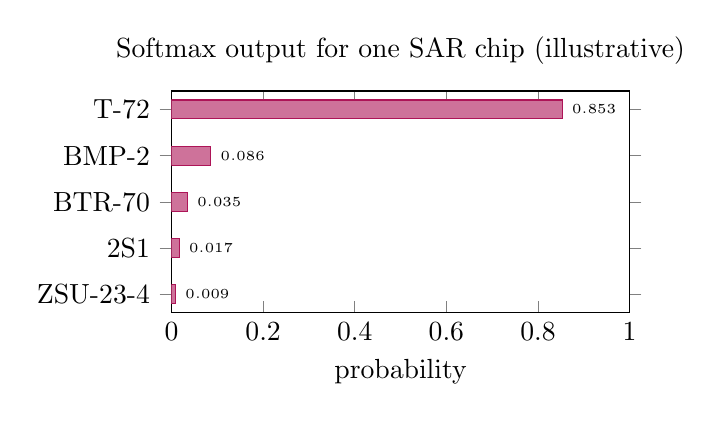
\begin{tikzpicture}
\begin{axis}[width=7.4cm,height=4.4cm,xbar,bar width=0.24cm,xmin=0,xmax=1,ytick=data,yticklabels={T-72,BMP-2,BTR-70,2S1,ZSU-23-4},y dir=reverse,xlabel={probability},title={Softmax output for one SAR chip (illustrative)},nodes near coords,nodes near coords style={font=\fontsize{5.5}{6.5}\selectfont,/pgf/number format/.cd,fixed,precision=3}]
\addplot[fill=AccentCol!60,draw=AccentCol] coordinates{(0.853,1)(0.086,2)(0.035,3)(0.017,4)(0.009,5)};
\end{axis}
\end{tikzpicture}}
\scriptsize Logits $(4.1,\,1.8,\,0.9,\,0.2,\,-0.4)$ for the top five classes $\to$ softmax.
\begin{cbox}{Loss}\scriptsize Categorical cross-entropy: $L=-\ln P(\text{true class})$. If the chip is a T-72: $L=-\ln0.853=0.159$.\end{cbox}
\column{0.47\textwidth}
\begin{cbox}[ISSAnavy]{Backpropagation through a conv layer}\scriptsize The same chain rule as before. Because one kernel is used at every position, its gradient is the \emph{sum} of contributions from all positions:
\[\frac{\partial L}{\partial K_{m,n}}=\sum_{i,j}\delta_{i,j}\,x_{i+m,\,j+n}\]
--- itself a convolution of the input with the error map. Max-pooling passes the gradient only to the winning pixel.\end{cbox}
\begin{cbox}{Training tricks}
\begin{tl}
\item \textbf{Data augmentation}: rotate, flip, shift, add noise --- free extra examples
\item \textbf{Batch normalisation}: stabilises activations, speeds training
\item \textbf{Dropout}: randomly silences units to reduce over-fitting
\end{tl}
\end{cbox}
\end{columns}
\end{frame}

%====================================================================
\sect{7. Architectures}
\begin{frame}{Landmark CNN Architectures}
\figc{2.3cm}{%
\begin{tikzpicture}[x=2.5cm]
\draw[ISSAnavy,line width=1pt,-{Stealth}] (0,0)--(5.3,0);
\foreach \x/\yr/\nm/\sub in {0.2/1998/LeNet-5/{digits; $\sim$60K params},1.3/2012/AlexNet/{ImageNet; $\sim$60M; GPUs, ReLU},2.4/2014/VGG-16/{all $3\times3$; 138M},3.5/2014/GoogLeNet/{Inception modules},4.6/2015/ResNet/{152 layers; skip links}}{%
 \fill[AccentCol] (\x,0) circle (3pt);
 \node[font=\scriptsize\bfseries,above=3pt] at (\x,0) {\yr};
 \node[nd,below=6pt,font=\fontsize{6}{7}\selectfont,text width=2.1cm] at (\x,0) {\textbf{\nm}\\\sub};}
\end{tikzpicture}}
\vspace{2pt}
\begin{columns}[T]
\column{0.48\textwidth}
\begin{cbox}{The 2012 turning point}\scriptsize AlexNet cut ImageNet top-5 error to 15.3\% against 26.2\% for the next-best entry. Three years later ResNet ensembles reached 3.57\%. Computer vision switched to deep learning almost overnight.\end{cbox}
\column{0.48\textwidth}
\begin{cbox}{ResNet's residual block}
\figc{1.4cm}{%
\begin{tikzpicture}[node distance=0.3cm]
\node[ndA] (x) {$x$}; \node[ndC,right=of x] (c1) {conv-BN-ReLU}; \node[ndC,right=of c1] (c2) {conv-BN}; \node[ndY,right=of c2] (p) {$+$}; \node[ndA,right=of p] (o) {ReLU};
\draw[arr] (x)--(c1); \draw[arr] (c1)--(c2); \draw[arr] (c2)--(p); \draw[arr] (p)--(o);
\draw[arrA,rounded corners] (x.north)--++(0,0.35)-|node[lab,pos=0.25,above]{identity shortcut}(p.north);
\end{tikzpicture}}
\scriptsize Output $=F(x)+x$: the same skip connection used in every Transformer block.\end{cbox}
\end{columns}
\end{frame}

\begin{frame}{Transfer Learning: When Labelled Military Data Is Scarce}
\begin{columns}[T]
\column{0.52\textwidth}
\figc{3.2cm}{%
\begin{tikzpicture}[node distance=0.3cm]
\node[ndG,minimum width=2.4cm] (src) {millions of everyday\\photos (ImageNet)};
\node[ndC,below=0.5cm of src,minimum width=2.4cm] (bb) {pre-trained\\convolutional backbone};
\node[ndN,right=1.4cm of bb,minimum width=2.2cm] (head) {new head:\\10 vehicle classes};
\node[ndY,above=0.5cm of head,minimum width=2.2cm] (tgt) {a few thousand\\labelled target chips};
\draw[arr] (src)--node[lab,right]{learn general edges, textures}(bb);
\draw[arr] (bb)--node[lab,above]{reuse}(head);
\draw[arr] (tgt)--node[lab,right]{train}(head);
\end{tikzpicture}}
\begin{cbox}{Two options}
\begin{tl}
\item \textbf{Feature extraction}: freeze the backbone; train only the new head --- fast, works with very little data
\item \textbf{Fine-tuning}: also update the later backbone layers with a small learning rate --- better when more data exist
\end{tl}
\end{cbox}
\column{0.45\textwidth}
\begin{rbox}\scriptsize\textbf{Why it works:} early-layer features (edges, corners, textures) are generic. Only the top layers are specific to the original task.\end{rbox}
\begin{wbox}\scriptsize\textbf{Caution for SAR:} radar imagery looks very different from optical photos (speckle, shadows, layover). The benefit of optical pre-training is smaller and must be checked on held-out SAR data.\end{wbox}
\begin{ibox}\scriptsize Synthetic training data from simulators and CAD models of vehicles is a common supplement --- but beware the gap between simulated and real returns (distribution shift, Lecture~1).\end{ibox}
\end{columns}
\end{frame}

%====================================================================
\sect{8. Defence Applications}
\begin{frame}{CNNs in Defence and Wargaming}
\begin{columns}[T]
\column{0.49\textwidth}
\begin{cbox}{Automatic target recognition (ATR)}\scriptsize Classifying vehicles in SAR chips. On the public MSTAR benchmark (10 vehicle classes) published CNNs report accuracies above 95\% under standard test conditions.\end{cbox}
\begin{cbox}{Object detection in EO/IR imagery}\scriptsize Detectors such as Faster R-CNN and YOLO output a box and a class for every object --- aircraft on aprons, ships in harbour, vehicles on roads.\end{cbox}
\begin{cbox}{Change detection and segmentation}\scriptsize Compare satellite images over time; label every pixel (road, building, crater) to update terrain databases for simulations.\end{cbox}
\column{0.48\textwidth}
\begin{cbox}{Wargaming and simulation}\scriptsize The map is an image: CNN policies read unit positions, terrain and visibility layers as channels (the approach used in game-playing systems such as AlphaGo).\end{cbox}
\begin{cbox}{Beyond images}\scriptsize 1-D CNNs on radar pulses, acoustic and RF signals (emitter identification); spectrograms treated as images.\end{cbox}
\begin{ibox}\scriptsize ``Standard conditions'' means test vehicles similar to training ones. Accuracy drops sharply for new depression angles, configurations or camouflage --- always ask how the test set was built.\end{ibox}
\end{columns}
\end{frame}

\begin{frame}{Failure Modes Every Analyst Must Know}
\begin{columns}[T]
\column{0.49\textwidth}
\begin{wbox}\textbf{Adversarial examples.}\ \scriptsize Tiny, invisible pixel changes can flip a prediction with high confidence (Goodfellow et al., 2014: a panda classified as a gibbon). Physical versions --- printed patches --- have fooled detectors in field tests.\end{wbox}
\begin{wbox}\textbf{Shortcut learning.}\ \scriptsize A network may key on background, sensor artefacts or image borders instead of the target. A frequently retold (and probably apocryphal) story describes a ``tank detector'' that had learned the weather in the photos --- the lesson is real even if the story is not.\end{wbox}
\column{0.48\textwidth}
\begin{wbox}\textbf{Distribution shift.}\ \scriptsize New sensor, season, terrain or decoys: performance can collapse with no warning, because softmax confidence stays high.\end{wbox}
\begin{cbox}{Checking what the CNN looks at}\scriptsize Saliency methods such as Grad-CAM colour the pixels that most influenced a decision. If the ``hot'' region is the background, not the vehicle, the model is not trustworthy --- whatever its accuracy.\end{cbox}
\begin{rbox}\scriptsize\textbf{Mitigations:} diverse training data, adversarial training, test sets from new conditions, and a human analyst confirming high-consequence calls.\end{rbox}
\end{columns}
\end{frame}

\begin{frame}{CNNs and Transformers Compared}
\centering\footnotesize\renewcommand{\arraystretch}{1.35}
\begin{tabularx}{\textwidth}{>{\bfseries}p{3.0cm} X X}
\toprule
& \textbf{CNN} & \textbf{Vision Transformer (ViT)}\\\midrule
Basic operation & convolution: fixed local window & self-attention: every patch to every patch\\
Built-in assumption & nearby pixels matter; same pattern anywhere & none --- relations learned from data\\
Data needed & works well on small/medium datasets & usually needs large datasets or pre-training\\
Long-range context & only through depth & from the first layer\\
Cost vs image size & linear in pixels & quadratic in number of patches\\
Shared ideas & \multicolumn{2}{p{0.68\textwidth}}{dot-product similarity, ReLU-type non-linearities, residual connections, softmax + cross-entropy, backpropagation}\\
\bottomrule
\end{tabularx}
\vspace{4pt}
\begin{ibox}\scriptsize In practice many current vision systems are hybrids: a CNN front end for local features feeding attention layers for global context. For small, specialised defence datasets, CNNs remain a strong and economical first choice.\end{ibox}
\end{frame}

\begin{frame}{Common Misconceptions}
\begin{columns}[T]
\column{0.49\textwidth}
\begin{wbox}\textbf{``Engineers design the filters.''}\ \scriptsize All kernel values are learned by backpropagation; hand-made edge filters are only a teaching device.\end{wbox}
\begin{wbox}\textbf{``Pooling is learned.''}\ \scriptsize Max and average pooling have no parameters.\end{wbox}
\begin{wbox}\textbf{``A $3\times3$ filter looks at 9 numbers.''}\ \scriptsize It looks at $3\times3\times C_{\text{in}}$ numbers --- all input channels at once.\end{wbox}
\column{0.49\textwidth}
\begin{wbox}\textbf{``CNNs are fully shift-invariant.''}\ \scriptsize Only approximately; small shifts can still change outputs, and rotations and scale changes need augmentation.\end{wbox}
\begin{wbox}\textbf{``High softmax = reliable.''}\ \scriptsize CNNs are often over-confident, especially on inputs unlike their training data.\end{wbox}
\begin{ibox}\scriptsize\textbf{Self-check:} if you can reproduce the four steps of the worked example and the parameter table, you understand the core of every CNN.\end{ibox}
\end{columns}
\end{frame}

\sect{9. Summary}
\begin{frame}{Summary and Quick Check}
\begin{columns}[T]
\column{0.55\textwidth}
\begin{fbx}{Convolution}$y_{i,j}=\sum_{m,n}K_{m,n}\,x_{i+m,j+n}+b$\end{fbx}
\begin{fbx}{Activation and pooling}$\text{ReLU}(z)=\max(0,z),\quad \text{maxpool: largest value per block}$\end{fbx}
\begin{fbx}{Output size}$n_{\text{out}}=\lfloor(n_{\text{in}}+2p-k)/s\rfloor+1$\end{fbx}
\begin{fbx}{Parameters per conv layer}$(k^2\,C_{\text{in}}+1)\,C_{\text{out}}$\end{fbx}
\begin{fbx}{Output}$P(\text{class})=\text{softmax}(W\,\text{GAP}(\text{features})+b)$\end{fbx}
\column{0.42\textwidth}
\begin{cbox}{Quick check}
\begin{te}
\item In the worked example, what is the output at position (1,0) for $K_1$, and why?
\item A $128\times128$ input meets a $5\times5$ kernel with $p=2$, $s=2$. What is the output size?
\item How many parameters has a layer of 256 filters of $3\times3$ on 128 input channels?
\item Why does a uniform bright region give 0 with an edge kernel?
\item Name two ways an adversary could defeat a CNN-based target recogniser.
\end{te}
\end{cbox}
\end{columns}
\end{frame}


\begin{frame}{Looking Ahead --- Lecture 8: Transformers, Intuitively}
\begin{columns}[T]
\column{0.50\textwidth}
\subhead{From pixels to words: models that read in context}
\begin{tl}\item What a language model does: one token at a time\item Embeddings as coordinates on a ``meaning map''\item Why one fixed vector per word fails --- the ``battery'' problem\item Encoder and decoder: who reads, who writes\item Attention as a radio net: queries, keys, values --- one computed by hand\item Multi-head attention, residuals, normalisation, cross-attention\end{tl}
\begin{ibox}\scriptsize\textbf{Assignment 7:} convolution, ReLU and pooling by hand + output-size formula + parameter counts for a CNN + receptive fields + an evaluation brief for a SAR recogniser; bonus: gradients through max-pooling and a shared kernel.\end{ibox}
\column{0.46\textwidth}
\begin{cbox}{Preview: one word, many meanings}\scriptsize ``The \emph{battery} was out of charge'' and ``the \emph{battery} opened fire'' use the same word for a power cell and an artillery unit. A transformer gives each occurrence a different vector, built from the words around it.\end{cbox}
\begin{rbox}\scriptsize A convolution scores a kernel against a patch with a dot product. Attention scores one word against another with the same dot product --- but the ``kernel'' is chosen by the data.\end{rbox}
\end{columns}
\end{frame}
\end{document}
